% !TEX spellcheck = en
\documentclass[main.tex]{subfiles} 

\begin{document}

\section{Tensor Fields}
\label{sec:2}
Our focus in this thesis is visualization of sceond order tensors in $\mathbf{R}^2$ and
$\mathbf{R}^3$. However, the theory we present in the following subsections will not 
be curtailed to second order tensors, but will be applicable to any order tensor field. 
In order to achieve this, we require a general notation. In this chapter, we first introduce 
the definition of a tensor of type $(M,N)$. Using this definition we show how 
tensors can be differentiated. We require this in order to introduce the Riemann Christoffel 
tensor; also known as Riemann curvature tensor, which quantifies the relative variation
of initially parallel geodesics \cite{Moo10}. Since such geodesics only variate relative
to each other in a curved space, the Riemann tensor will be zero everywhere in flat space.

%%%%%%%%%%%%%%%%%%% Notation %%%%%%%%%%%%%%%%%
\subsection{Notation}
Here we provide a short introduction to Einstein notation, which we will employ throughout
this thesis.

In an orthogonal coordinate system we can write a vector $\mathbf{A}$ in component form
\begin{align*}
\mathbf{A} = A_1 \hat{e}_1 + A_2 \hat{e}_2 + A_3 \hat{e}_3,
\end{align*}
where $\hat{e}_i,\; i=1,2,3$ are the orthogonal unit vectors. The short hand notation we 
just employed for the orthogonal vectors uses a dummy subscript $i$. Using this subscript, 
we can achieve a shorter notation, also called the \emph{index} notation :
\begin{align*}
A_i, \;i = 1,2,3.
\end{align*}
Here $A_i$ refers to all the components of the vector\footnote{As a single subscript/superscript 
denotes the components of a vector, we can extend this to higher(or lower) order systems. 
No subscript or superscript denote scalars, which we refer to as zeroth-order systems. While 
two indices imply a second order system, which in the language of linear algebra is called a 
matrix (if the indices are not mixed). We will, however, refer to such systems as tensors. 
In fact, nomenclature tensor is the unified reference to all such systems, and those of higher order.}
$\mathbf{A}$. 

To avoid confusion, a system of any order when raised to a power will be enclosed
in paranthesis
\begin{align*}
(B^2)^3, (y_1^{\phantom{1}1})^2, (T_{ij}^{\phantom{ij}kl})^{1/2} .
\end{align*}
Hence, the component $B^2$ is raised to the power of 3, the component 
$y_1^{\phantom{1}1}$ is raised to the power of 2, and for the tensor $T_{ij}^{\phantom{ij}kl}$ 
we take the square root\footnote{Which is not as simple or straight forward as it sounds. 
In order for any mathematical operation to be performed on a tensor, the resulting tensor 
must obey the transformation law. We will discuss this later when we introduce the 
general definition of tensors.}. 

When a system has indices that occur unrepeated, it is implicitly understood that each of
the subscripts and superscripts can take any of the integer values $1,\hdots,N$. For example
the \emph{Kronecker delta} symbol $\delta_{ij}$, defined by
\begin{align} \label{eq:Kroncker_delta}
\delta_{ij} = &
\left\{\begin{matrix}
 1 & \mbox{for } i=j \\
 0 & \mbox{for } i \neq j,
\end{matrix}\right.
\end{align}
with $i,j = 1,2,3$, represents nine values.
The indices $i$ and $j$ are called \emph{free indices} and can take on any of the values specified 
by a given range. 

\emph{The summation convention} states that when an index which is repeated twice on the same 
side of an equation, it is understood to represent a summation of the repeated indices. Hence,
a repeated index is called a \emph{summation index}, while an unrepeated index is called a
\emph{free index}.
To sum the diagonal entries of the Kroncker delta\footnote{In linear algebra this is referred 
to as taking the \emph{trace} of an $n\times n$ square matrix.}, we simply repeat the indices
\begin{align*}
\delta_{ii} = \delta_{11} + \delta_{22} + \delta_{33} = 3.
\end{align*}
Note that we implicitely understand, when we write $\delta_{ii}$, to mean that we are performing
the summation
\begin{align*}
\sum\limits_i^3 \delta_{ii}.
\end{align*}

Often when performing certain operations, the alternating tensor becomes a handy tool to
possess. It is a short-hand notation, just like the Kronecker delta. 
\begin{mydef}
The e-permutation sysmbol is defined as 
\end{mydef}
\begin{align*}
e_{ijk} = &
\left\{\begin{matrix}
 1 & \mbox{if }  ijk \mbox{ is an even permutation}, \\
-1 & \mbox{if } ijk \mbox{ is an odd permutation}, \\
 0 & \mbox{when indices overlap}.
\end{matrix}\right.
\end{align*}
The definition is also applicable for larger sets as well. 
Another identity which is useful, is the e-$\delta$ identity. Given $e_{ijk}$ the 
e-permutation symbol, and $\delta_{ij}$ the Kronecker delta, then for $i, j, k, m, n = 
1, 2, 3$,
\begin{align*}
e_{ijk} e_{imn} = \delta_{jm} \delta_{kn} - \delta_{jn} \delta_{km},
\end{align*}
where i is the summation index and j, k, m, n are the free indices. A mixed superscript
and subscript identity, is defined as
\begin{align*}
e^{ijk} e_{imn} = \delta^j_{\phantom{j}m} \delta^k_{\phantom{k}n} - 
			   \delta^j_{\phantom{j}n} \delta^k_{\phantom{j}m}
\end{align*}
Using the e-permutation symbol we can describe the determinant of a tensor A with the
components  $a_{ij}$, where $i, j = 1, \dots, n$. Writing the determinant in index notation, 
it becomes
\begin{align*}
det A = \|A\| = e_{{i_1}\dots{i_n}} a_{1{i_1}}\dots a_{n{i_n}}
\end{align*} 
For a $3\times3$ matrix,
\begin{align*}
det A &= e_{ijk} a_{1i}a_{1j}a_{1k} \\
	 &= e_{1jk} a_{11}a_{1j}a_{1k} + e_{2jk} a_{12}a_{1j}a_{1k} + e_{3jk} a_{13}a_{1j}a_{1k} \\
         &= e_{123} a_{11}a_{12}a_{13} + e_{132} a_{11}a_{13}a_{12}
	    + e_{213} a_{12}a_{11}a_{13}  + e_{231} a_{12}a_{13}a_{11}
	    + e_{312} a_{13}a_{11}a_{12} + e_{321} a_{13}a_{12}a_{11} \\
	&= a_{11}a_{12}a_{13} - a_{11}a_{13}a_{12}
	     - a_{12}a_{11}a_{13}  + a_{12}a_{13}a_{11}
	    + a_{13}a_{11}a_{12} - a_{13}a_{12}a_{11}
\end{align*} 
This is a simple illustration for the need of using short hand notation.

%%%%%%%%%%%%%%%     General Definition of Tensor    %%%%%%%%%%%%%%%

\subsection{A General Definition of Tensor}
We now introduce a definition of a tensor field, evaluated at a point $x^j = x^j(\bar{x}^j)$. 
The bar quantity are coordinates in different coordinate system. We assume that a mapping exists, 
such that $\bar{x}^j = \bar{x}^j(x^j)$. We define the transformation between the barred 
coordinate system and the barless coordinates as
\begin{align}
\label{eq:trans}
\bar{x}^j = \bar{x}^j(x^j).
\end{align}

\begin{mydef}
A tensor of rank $(M+N)$,
$\mathcal{T}^{\phantom{i_1 \hdots i_M}j_1 \hdots j_N}_{\,\,i_1 \hdots i_M}(x^j)$, defined on a point P of 
a differential manifold $X_n$ exists, if, under the coordinate transformation \eqref{eq:trans}, 
the components transform according to the law
\begin{align} \label{def:tensor}
\overline{\mathcal{T}}^{\phantom{m_1 \hdots m_N}n_1 \hdots n_N}_{m_1 \hdots m_M} = 
\frac{\partial x^{i_1}}{\partial \bar{x}^{m_1}} \cdot \hdots \cdot 
\frac{\partial x^{i_M}}{\partial \bar{x}^{m_M}} \cdot
\frac{\partial \bar{x}^{n_1}}{\partial x^{j_1}}  \cdot \hdots \cdot 
\frac{\partial \bar{x}^{n_N}}{\partial x^{j_N}}
\mathcal{T}^{\phantom{i_1 \hdots i_M}j_1 \hdots j_N}_{\,\,i_1 \hdots i_M}.
\end{align}
The tensor is said to be \emph{covariant} of order M and \emph{contravariant} of order N, 
if it obeys the \emph{transformation law}.
\end{mydef}

\begin{example}
Let $\phi = \phi(x^1,\hdots,x^N)$ denote a tensor of type $(0,0)$. Then from 
Equation (\ref{def:tensor}) it follows that
\begin{align*}
\bar{\phi}(\bar{x}^1,\hdots,\bar{x}^N) = \phi(x^1,\hdots,x^N).
\end{align*}
This is simply a scalar. Hence scalars are zero order tensors. The gradient of the scalar 
is another tensorial quantity. By chain rule, 
\begin{align*}
\frac{\partial \bar{\phi}}{\partial\bar{x}^j} = \frac{\partial x^i}{\partial \bar{x}^j}
          															  \frac{\partial\phi}{\partial x^i}									
\end{align*}
which we see is a covariant vector of type (1,0). 
\end{example} 
In general, we can write such vectors by the transformation law.
\begin{align*}
\bar{A}_j = \frac{\partial x^i}{\partial \bar{x}^j} A_i.
\end{align*}
Similarly, a contravariant vector is a type (0,1) tensor, and by the transformation law
given as
\begin{align*}
\bar{A}^j = \frac{\partial \bar{x}^j}{\partial x^i} A^i.
\end{align*}

The importance of tensors is made clear due to the fact that they are invariant under coordinate 
transformations. Hence, if all the components of the tensor vanish in one coordinate system, 
they will do so in any other system. Similarly, if the tensor is symmetric in one coordinate system, 
the property will perpetuate on to another coordinate system.
\begin{proof}
Given the tensor $R_{ijk}$, it is said to be symmetric in two of its indices if the components are 
unchanged when the indices are interchanged. For example, the third order tensor $R_{ijk}$ is 
symmetric in the indices $i$ and $k$, if
\begin{align} \label{eq:R_symm}
R_{ijk} = R_{kji}
\end{align}
for all values of $i,j$ and $k$. By the transformation law (\ref{def:tensor}),
\begin{align} \label{eq:R_lmn}
\overline{R}_{lmn}= \frac{\partial x^i}{\partial \bar{x}^l} 
						  \frac{\partial x^j}{\partial \bar{x}^m} 
						  \frac{\partial x^k}{\partial \bar{x}^n} R_{ijk},
\end{align}
and
\begin{align*}
\overline{R}_{nml}= \frac{\partial x^k}{\partial \bar{x}^n} 
						  \frac{\partial x^j}{\partial \bar{x}^m} 
						  \frac{\partial x^i}{\partial \bar{x}^l} R_{kji}.
\end{align*}
By Equation \eqref{eq:R_symm} and \eqref{eq:R_lmn} it follows that
\begin{align*}
\overline{R}_{nml} = \frac{\partial x^k}{\partial \bar{x}^n} 
						  \frac{\partial x^j}{\partial \bar{x}^m} 
						  \frac{\partial x^i}{\partial \bar{x}^l} 
				   \left(\frac{\partial \bar{x}^l}{\partial x^i}
						  \frac{\partial \bar{x}^m}{\partial x^j}
						  \frac{\partial \bar{x}^n}{\partial x^k} \overline{R}_{lmn}
						  \right)
						= 	\overline{R}_{lmn},
\end{align*}
where we used the inverse relation of Equation \eqref{eq:R_lmn}.
\end{proof}
A tensor is skew-symmetric in two of its indices if the components are transformed to 
their negative values when the indices are interchanged. Using $R_{ijk}$ again to 
illustrate this,
\begin{align*}
R_{ijk} = -R_{kji}
\end{align*}
for all values of $i,j$ and $k$. Using the proof above, we can readily show for a 
skew-symmetric tensor the property of invariance from one coordinate system to 
another.



\subsection{Tensor Operations}
In order for an operation to make sense when performed on a tensor, the resulting 
tensor must satisfy the transformation law (\ref{def:tensor}).
\begin{example}
We can add or subtract similar components for different tensors. The following operation is 
permitted only when the indices match 
\begin{align} \label{eq:valid}
C^i_{\phantom{i}jk} = A^i_{\phantom{i}jk} + B^i_{\phantom{i}jk}.
\end{align}
This is invalid
\begin{align} \label{eq:invalid}
A^i + B_j.
\end{align}
For \eqref{eq:invalid}, the system B is a covariant of order 1, while system A is 
contravariant of order 1. 

We can show that the operation performed in \eqref{eq:valid} 
is correct by employing the transformation law. It is a good way to show that a certain 
tensor operation is valid. Let A and B be expressed by the transformation law (\ref{def:tensor})
\begin{align}
\bar{A}^l_{\phantom{l}mn} = 
\frac{\partial\bar{x}^l}{\partial x^i}\frac{\partial x^j}{\partial\bar{x}^m}
\frac{\partial x^k}{\partial\bar{x}^n} A^i_{\phantom{i}jk},
\end{align}
and,
\begin{align}
\overline{B}^l_{\phantom{l}mn} = 
\frac{\partial\bar{x}^l}{\partial x^i}\frac{\partial x^j}{\partial\bar{x}^m}
\frac{\partial x^k}{\partial\bar{x}^n}B^i_{\phantom{i}jk}.
\end{align}
Then,
\begin{align*}
 \overline{C}^l_{\phantom{l}mn} = A^l_{\phantom{l}mn} + B^l_{\phantom{l}mn} &= 
\frac{\partial\bar{x}^l}{\partial x^i}\frac{\partial x^j}{\partial\bar{x}^m}
\frac{\partial x^k}{\partial\bar{x}^n} \left(A^i_{\phantom{i}jk} + B^i_{\phantom{i}jk}\right)
= \frac{\partial\bar{x}^l}{\partial x^i}\frac{\partial x^j}{\partial\bar{x}^m}
\frac{\partial x^k}{\partial\bar{x}^n} C^i_{\phantom{i}jk}.
\end{align*}
Which clearly satisfies the transformation law. 

For the case in \eqref{eq:invalid}, 
we can use same procedure to demonstrate that the quantity is not tensorial.
In general, we can say that only tensors of same type $(r,s)$ can be added together.
\\

Multiplication (outer product) on the other hand does not require tensors have the exact 
same type. For example the outer product of the systems $A^{\phantom{m}i}_m$ and 
$B^{jkl}$ result in the new system
$C_m^{\phantom{m}ijkl}$,
\begin{align*}
C_{m}^{\phantom{m}ijkl} = A^{\phantom{m}i}_mB^{jkl}.
\end{align*}
The newly constructed system from the outer product is a fifth order system, consisting of all 
the possible products from the components of $A^{\phantom{m}i}_m$ with $B^{jkl}$. 
\\

The operation of contraction occurs when the lower and upper index are set equal to each other
and the summation convention is thereby applied. Using the system $C_m^{\phantom{m}ijkl}$ 
from the previous example, we can perform contraction on the lower index n with the upper 
index i as following
\begin{align*}
C^{\phantom{m}mjkl}_{m} = C^{\phantom{1}1jkl}_{1} + \dots + C^{\phantom{N}Njkl}_{N}
= D^{jkl}
\end{align*}
where we have summed the same indices through the summation convention. As a result of 
contracting the system C, the resulting system is now a third order system. In fact, performing
contraction on a system always lowers the order of the system by two. 
\\

An \emph{inner product} between two tensors is performed as following. Firstly, take the 
outer product of the tensor, thereafter perform a contraction on two of the indices. As 
contraction requires both super and sub-script, the tensors involved in such an operation 
must be at least of rank 1. Given two vectors $A^i$ and $B_j$, their inner product is found 
by first performing an outer product
\begin{align*}
C^i_{\phantom{i}j} = A^i B_j.
\end{align*}
Thereupon, we perform a contraction by setting the indices equal to each other, and sum all the
terms. Using the transformation law for the contravariant tensor $A^i$ and covariant tensor
$B_j$, they take the form
\begin{align*}
\bar{A}^i &= \frac{\partial \bar{x}^j}{\partial x^m} A^m,\\
\overline{B}_j &= \frac{\partial x^n}{\partial \bar{x}^j} B_n.
\end{align*}
There upon we perform the product
\begin{align*}
\bar{A}^i\overline{B}_j &= \left(\frac{\partial \bar{x}^j}{\partial x^m} A^m\right)
 \left(\frac{\partial x^n}{\partial \bar{x}^j} B_n\right), \\
 \bar{A}^i\overline{B}_j &=  \frac{\partial \bar{x}^j}{\partial x^m}
 							 \frac{\partial x^n}{\partial \bar{x}^j}
 							 A^m B_n.					  
\end{align*}
Let $\overline{C} = \bar{A}^i\overline{B}_i$, then the contraction by setting $i=j$ and
summing all the terms, becomes
\begin{align*}
\overline{C} &= \bar{A}^i\overline{B}_i,\\
			 &= \delta^n_{\phantom{n}m} A^m B_n,\\
			 &= A^n B_n	= C.
\end{align*}
As we observe, the end result becomes a scalar (as implied by the terminology - scalar product).
\end{example}


%%%%%%%%  Reciprocal Basis and Metric Tensor %%%%%%%%%%
\subsection{Reciprocal Basis and the Metric Tensor}
\label{sec:metric}
\begin{mydef}
Two bases $(\mathbf{E}_1,\mathbf{E}_2,\mathbf{E}_3)$ and $(\mathbf{E}^1,\mathbf{E}^2,
\mathbf{E}^3)$ are said to be reciprocral if they satisfy the condition
\begin{align*}
E_iE^j = \delta^{\phantom{i}j}_i = 
\left\{\begin{matrix}
 1 & \mbox{for } i=j \\
 0 & \mbox{for } i \neq j
\end{matrix}\right.
\end{align*}
\end{mydef}
One such basis that satisfies this is
\begin{align*}
E_i = \frac{\partial \mathbf{r}}{\partial u^i}
\end{align*}
where $\mathbf{r} = x(u,v,w)\mathbf{e}_1 + y(u,v,w)\mathbf{e}_2 + z(u,v,w)\mathbf{e}_3$.
The unit vectors $e_i$ are defined as $\frac{E_i}{\left|E_i\right|}$.
Given the basis $(\mathbf{E}_1,\mathbf{E}_2,\mathbf{E}_3)$, we can always 
determine $(\mathbf{E}^1,\mathbf{E}^2,\mathbf{E}^3)$ by the following triple 
scalar products
\begin{align*}
E^i = \frac{e_{ijk}E_j E_k}{e_{ijk}E_iE_jE_k}.
\end{align*}
Given these new basis vectors, 
we can now represent any vector, $\mathbf{A}$, by either of the baseis. Given the basis 
$(\mathbf{E}_1,\mathbf{E}_2,\mathbf{E}_3)$, we can represent $\mathbf{A}$ in the form
\begin{align*}
A^i E_i.
\end{align*}
The components of $\mathbf{A}$, $A^i$, relative to basis $E_i$ are called 
\emph{contravariant components} of $\mathbf{A}$. 
Similarly, the components $A_i$ relative to the basis $E^i$ are called 
\emph{covariant components} of $\mathbf{A}$ :
\begin{align*}
A_i E^i.
\end{align*}
The contra and co-variant are different ways of representing $\mathbf{A}$ with respect to 
a set of reciprocal basis vectors. The inter-relationship between these components is given 
by the \emph{metric} and the \emph{cojugate metric} of space
\begin{align*}
g_{ij} &= E_iE_j = \frac{\partial \mathbf{r}}{\partial u^i} \cdot \frac{\partial \mathbf{r}}{\partial u^j}, \\
g^{ij} &= E^iE^j = (g_{ij})^{-1},
\end{align*}
where the last identity follows from the reciprocity.
In index notation, the relationship expressed with the metric becomes
\begin{align*}
A_i = g_{ij}A^j, \\
A^i = g^{ij}A_j.
\end{align*}
Hence, we can both raise the indices, and lower them, by applying either the 
conjugate metric $g^{ij}$ or the metric $g_{ij}$. This is an useful operation 
(e.g. when applied to higher-order tensors like the Riemann curvature tensor.)

Let $x = x(u,v,w), y = y(u,v,w), z = z(u,v,w)$, then the curve element $ds$ is given as
\begin{align*}
ds^2 = g_{ij}du_idu_j.
\end{align*}

An example of this is illustrated by transforming the Cartesian coordinates $(x,y,z)$ to 
cylindrical $(r,\theta,z)$. The relationship between these coordinate systems is as following
\begin{align*}
x &= r\cos(\theta),\\
y &= r\sin(\theta),\\
z &= z. 
\end{align*}
Hence, $x$, $y$, and $z$ are functions of $u_i = (r,\theta,z)$, and the line vector $\mathbf{r}$ is given as
$\mathbf{r} = x(r,\theta,z)\mathbf{e}_1 + y(r,\theta,z)\mathbf{e}_2 + z(r,\theta,z)\mathbf{e}_3$.
The the non-zero entries of the metric are the diagonal entries
\begin{align*}
g_{11} = \frac{\partial \mathbf{r}}{\partial r} \cdot \frac{\partial \mathbf{r}}{\partial r},  \qquad
g_{22} =\frac{\partial \mathbf{r}}{\partial \theta} \cdot \frac{\partial \mathbf{r}}{\partial \theta}, \qquad
g_{33} = \frac{\partial \mathbf{r}}{\partial z} \cdot \frac{\partial \mathbf{r}}{\partial z}.
\end{align*}
The non-zero calcuated entries of the metric are given as
\begin{align*}
g_{11} &= \left[\cos(\theta)\mathbf{e}_1 + \sin(\theta)\mathbf{e}_2\right] \cdot  
	        \left[\cos(\theta)\mathbf{e}_1 + \sin(\theta)\mathbf{e}_2\right] = 1,\\
g_{22} &= \left[-r\sin(\theta)\mathbf{e}_1 + r\cos(\theta)\mathbf{e}_2\right] \cdot  
	        \left[-r\sin(\theta)\mathbf{e}_1 + r\cos(\theta)\mathbf{e}_2\right]  = r^2,\\
g_{33} &= \mathbf{e}_3 \cdot \mathbf{e}_3 = 1.
\end{align*}
The line element $ds$ thus becomes
\begin{align*}
ds^2 = dr^2 + r^2 d\theta^2 + dz^2. \qquad\qquad\qquad\phantom{.}
\end{align*}



%%%%%%%%%%% Tensor diffrerentiation %%%%%%%%%%%
\subsection{Tensor Differentiation}
Say that we want to differentiate a tensor field $T_{ij}(x^k)$, where $x^k = x^k(\bar{x}^k)$, as following
\begin{align*}
\frac{\partial T_{ij}}{\partial x^k}.
\end{align*}
We know now that this quantity has to satisfy the transformation law (\ref{def:tensor}).
The second order tensor of type $(2,0)$ satisfies the following transformation law
\begin{align*}
\overline{T}_{pq} = \frac{\partial x^i}{\partial \bar{x}^p}\frac{\partial x^j}{\partial \bar{x}^q} T_{ij}
\end{align*}
If we now perform differentiation on this expression, we get
\begin{align*}
\frac{\partial \overline{T}_{pq}}{\partial x^k} = 
\frac{\partial^2 x^i}{\partial x^k \partial \bar{x}^p}\frac{\partial x^j}{\partial \bar{x}^q} T_{ij} + 
\frac{\partial x^i}{\partial \bar{x}^p}\frac{\partial^2 x^j}{\partial x^k \partial \bar{x}^q} T_{ij} +
\frac{\partial x^i}{\partial \bar{x}^p}\frac{\partial x^j}{\partial \bar{x}^q}
\frac{\partial T_{ij}}{\partial x^k}.
\end{align*}
This quantity is certainly not a tensor. In order to derivate a tensor, we need to introduce
the Christoffel symbols.  

Consider the metric tensor $g_{ab}$ which satifies the transformation law
\begin{align} \label{eq:metric_g}
\overline{g}_{kl} = g_{ab} \frac{\partial x^a}{\partial \bar{x}^k}\frac{\partial x^b}{\partial \bar{x}^l}.
\end{align}
We define a quantity,
\begin{align} \label{eq:klm}
(k,l,m) = \frac{\partial \overline{g}_{kl}}{\partial \bar{x}^m}.
\end{align}
We insert \eqref{eq:metric_g} in \eqref{eq:klm}, and simply apply chain rule
\begin{align*}
(k,l,m) =   \frac{\partial g_{ab}}{\partial x^c} \frac{\partial x^c}{\partial x^m} 
	        \frac{\partial x^a}{\partial \bar{x}^k}\frac{\partial x^b}{\partial \bar{x}^l} + 
		g_{ab}\frac{\partial^2 x^a}{\partial x^m \partial \bar{x}^k}
	        \frac{\partial x^b}{\partial \bar{x}^l} +
		g_{ab}\frac{\partial x^a}{\partial \bar{x}^k}
	        \frac{\partial^2 x^b}{\partial x^m \partial \bar{x}^l}.
\end{align*}
By combining the terms, \cite{Hei01},
\begin{align*}
\frac{1}{2} \left[(k,l,m) + (l,m,k) - (m,k,l)\right]
\end{align*}
we can extract Christoffel symbol of \emph{first kind}, which is defined as
\begin{align} \label{eq:first_kind}
\frac{1}{2} \left[\frac{\partial g_{ab}}{\partial x^c} + \frac{\partial g_{bc}}{\partial x^a} -
                        \frac{\partial g_{ac}}{\partial x^b}\right].
\end{align}
By introducing a shorter notation \cite{Hei01}, we can write \eqref{eq:first_kind} as
\begin{align*}
[ac, b] = [ca,b].
\end{align*}
This implies that we have symmetry about the variables $a$ and $c$. 
This new quantity is not a tensor, as it does not satisfy the transformation law.
\\

Christoffel symbol of \emph{second kind} is defined as 
\begin{align*}
 g^{mb} \left[ac,b\right] = \frac{1}{2} g^{mb} \left[\frac{\partial g_{ab}}{\partial x^c} + 
								   \frac{\partial g_{bc}}{\partial x^a} -
                        					   \frac{\partial g_{ac}}{\partial x^b}\right].
\end{align*}
We can write this in a shorter notation by using brackets
\begin{align} 
\label{eq:second_kind}
{m\brace b\,\,c} = {m\brace c\,\,b} = g^{mb} \left[ac,b\right],
\end{align}
where we have symmetry between $b$ and $c$. This quantity is not a tensor either;
agian, it does not obey the transformation law. We can interchange between the 
second kind and first kind, by multiplying \eqref{eq:second_kind} with the metric 
$g_{mb}$. As $g_{mb}\,g^{mb} = \delta^{\phantom{m}b}_m$ (see Section 
\ref{sec:metric}), we end up with the Christoffel symbol of first kind, \eqref{eq:first_kind}.
\\

So far we have introduced new notation for derivating tensors, yet the operators 
themselves are not tensors\footnote{\cite{Hei01} purposely introduced the above 
notation as to clearly avoid any confusion between a tensor and Christoffel symbols.
Another oft-used symbols for Christoffel symbol of second kind is ${i \brace j\,\,k} = 
\Gamma^i_{jk}$. This notation is used for instance by \cite{LR89}, and many other 
authors.}. The purpose of Christoffel symbols becomes quite apparent, when 
we use these operators to define a covariant derivative of a tensor. 

The covariant derivative of a covariant tensor, $A_m$, is given as
\begin{align*}
A_{b, c} = \frac{\partial A_b}{\partial x^c} - {m\brace b\,\,c} A_m.
\end{align*}
which becomes a second order tensor, satisfying the transformation law
\begin{align*}
\bar{A}_{i,j} = A_{b, c} \frac{\partial x^b}{\partial \bar{x}^i} 
				   \frac{\partial x^c}{\partial \bar{x}^j}.
\end{align*}
We have sucessfully managed to derivate a tensor, and the resulting
operation adheres to the transformation law. In other words, the derivative 
of the tensor results in a another tensor. 
\\

Similary, we can show that the covariant derivative of the contravariant tensor $A^m$, 
\begin{align*}
A^m_{\phantom{m},n} = \frac{\partial A^m}{\partial x^n} + {m\brace l\,\,n} A^l
\end{align*}
obeys the transformation law. Here, the first term on the right hand side of the 
equation is the rate of the tensor field as we move along a coordinate curve, while 
the second term is the change in local basis vectors as we move along the coordinate 
curves, \cite{Hei01}.

For second order tensors $A_{ij}, A^i_{\phantom{i}j}, A^{ij}$, their covariant derivatives are
given as
\begin{align*}
A_{ij,k} &= \frac{\partial A_{ij}}{\partial x^k}  - 
				  A_{mj}{m \brace i\,\,k} - 
				  A_{im}{m \brace j\,\,k},\\ 
A^i_{\phantom{i}j,k} &= \frac{\partial A^i_{\phantom{i}j}}{\partial x^k}  + 
				 A^m_{\phantom{m}j}{i \brace m\,\,k} - 
				 A^i_{\phantom{i}m}{m \brace j\,\,k},\\
A^{ij}_{\phantom{ij},k} &= \frac{\partial A^{ij}}{\partial x^k}  + 
				   A^{mj}{i \brace m\,\,k} +
				   A^{im}{j \brace m\,\,k}.
\end{align*}
Given two tensors, say $A_{ij}$ and $B_{ij}$, the covariant derivation is same
as ordinary derivation, where
\begin{enumerate}
\item $(A_{ij} + B_{ij})_{,k} = A_{ij,k} + B_{ij,k}$ (derivative of sum is the sum of derivatives)
\vspace{-2mm}
\item $(A_{ij}B_{ij})_{,k} = A_{ij,k}B_{ij} + A_{ij}B_{ij,k}$ (product rule)
\vspace{-2mm}
\item $(A_{ij,k})_{,l} = A_{ij,kl}$ (higher-order derivatives are defined as derivatives)
\footnote{It is worth noting that unlike partial derivatives, where for example the second 
order derivative of a function f, $\frac{\partial^2 f}{\partial x^i\partial x^j} = \frac{\partial^2 f}
{\partial x^j\partial x^i}$. This does not necessarily apply for higher-order covariate 
derivatives of tensors, where in general $A_{i,jk} \neq A_{i,kj}.$}
\end{enumerate}
\vspace{3mm}We can now finally introduce the Riemann-Christoffel Tensor. The tensor is
found by the following identity
\begin{align}
A_{i,jk} - A_{i,kj} = A_m R^m_{\phantom{m}ijk},
\end{align}
where the fourth-order tensor
\begin{align}
\label{eq:RCT}
R^m_{\phantom{m}ijk} =  
\frac{\partial}{\partial x^j}{m \brace i\,\,k} - \frac{\partial}{\partial  x^k}{m \brace i\,\,j} + 
{n \brace i\,\,k}{m \brace n\,\,j} - {n \brace i\,\,j}{m \brace n\,\,k},
\end{align}
is called the Riemann-Christoffel tensor\footnote{Named after Bernhard Riemann and Elwin Bruno
Christoffel.}$\phantom{}^,$\footnote{Another way to introduce the Riemann curvature tensor is by using the 
geodesic differential equations. We will later introduce these when we discuss techniques for 
visualization of second order tensor fields.}, Riemann curvature tensor, or simply Riemann
tensor. The covariant form of the tensor can be found by multiplying the Riemann curvature tensor with the 
metric $g_{pm}$
\begin{align*}
R_{pijk} = g_{pm}R^m_{\phantom{m}ijk}.
\end{align*}
This tensor is skew-symmetric in two of it's indices
\begin{align*}
R_{pijk} &= - R_{pikj}\\
R_{jkpi} &= - R_{jkip}
\end{align*}
From the covariant Riemann-Christoffel tensor it follows that there are  
$N = \frac{1}{12} n^2 (n^2 - 1)$ independent components. For two-dimensions
there is only one independent component, while for three-dimensions there are
6 independent components

The tensor therefore provides a way for determining if the space is flat or curved.
If the Riemann tensor for a given spacetime is zero every where, initially any parallel
geodesics remain parallel (the spacetime is flat, otherwise the spacetime is curved).
\\

We may also define the Ricci tensor $R_{jk}$ by contracting the curvature tensor \eqref{eq:RCT},
\begin{align*}
R_{jk} = R^m_{\phantom{m}mjk} = g^{pi}R_{pijk}.
\end{align*}
When expressed with Christoffel symbols, we can show that the Ricci tensor is symmetric.
Performing another contraction, we get the scalar curvature
\begin{align*}
R = R^{j}_{\phantom{j}k} = g^{kj}R_{jk}.
\end{align*}
Since this quantity is invariant in any coordinate system, it gives a coordinate
independent measure of a space curvature. However, even though both the Ricci tensor 
and the scalar curvature can be zero in \emph{curved space}, a non-zero value clearly 
indicates that the space is curved. Which in it self is useful. Only by evaluating
the Riemann tensor can one conclusively distinguish flat and curved space \cite{Moo10}.

%%%%%%%%%%%% Curvature Tensor for Toroidal Coordinates %%%%%%%%%%%%%
\subsection{Example: Riemann Curvature Tensor for Toroidal Coordinates}

This coordinate system $(\eta, \theta , \psi)$ results from rotating a two-dimensional 
bipolar coordinate system about the axis that separates it's two foci. The coordinate 
relationship between toroidal and cartesian coordinate system is given as
\begin{align}
\label{eq:x_coord}
x &= \frac{a \sinh (\eta) \cos (\psi)}{\cosh (\eta) - \cos (\theta)} \\
\label{eq:y_coord}
y &= \frac{a \sinh (\eta) \sin (\psi)}{\cosh (\eta) - \cos (\theta)} \\
\label{eq:z_coord}
z &= \frac{a \sin (\theta)}{\cosh (\eta) - \cos (\theta)} 
\end{align}
where $\theta$ coordinate of a point P equals the angle $F_1 P F_2$, where $F_1$ and $F_2$
are the two foci as displayed below.

\begin{figure}[H]
\hspace{60mm}
\scalebox{.9}{
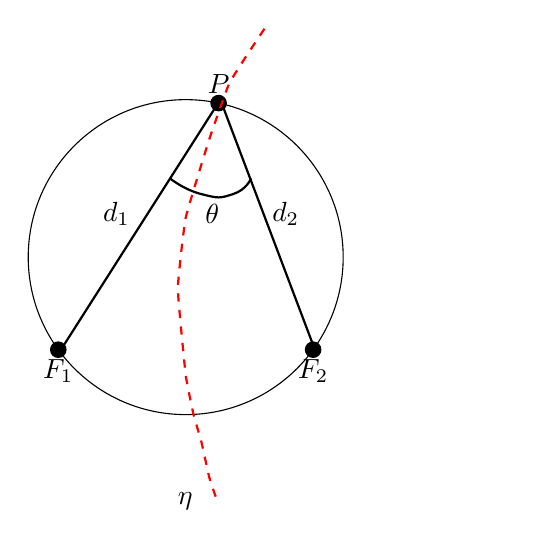
\begin{tikzpicture}
  \coordinate (center) at (3,2);
  \def\radius{2cm}
  \draw (center) circle[radius=\radius];
  \fill[black] (center) ++(1.2*180:\radius) circle[radius=3pt] node[below] {$F_1$};
  \fill[black] (center) ++(1.8*180:\radius) circle[radius=3pt] node[below] {$F_2$};
  \fill[black] (center) ++(0.433*180:\radius) circle[radius=3pt] node[above] {$P$};
  \draw[thick] (1.40,0.8) -- (3.44,4);
  \node[text width=3cm] at (3.45,2.55) {$d_1$};
  \draw[thick] (4.65,0.8) -- (3.44,4);
  \node[text width=3cm] at (5.6,2.55) {$d_2$};
  \draw[red,thick,dashed] plot [smooth, tension=0.2]  coordinates {(4, 4.9) (3.8, 4.6) (3.55,4.2) 
           (3.3,3.5) (3.0,2.5) (2.9,1.6) (3, 0.5) (3.1, 0)(3.2, -0.35)(3.3, -0.8)(3.4, -1.1)};
  \draw[thick] plot [smooth, tension=1]  coordinates {(2.8,3)(3.2,2.8)(3.6,2.8)(3.83,3)};
  \node[text width=3cm] at (4.75,2.55) {$\theta$};
  \node[text width=3cm] at (4.4, -1.1) {$\eta$};
\end{tikzpicture}}
\caption[Reference circle on a toroid.]{Reference circle on a toroid.}
\end{figure}

\begin{figure}[H]
\hspace{5mm}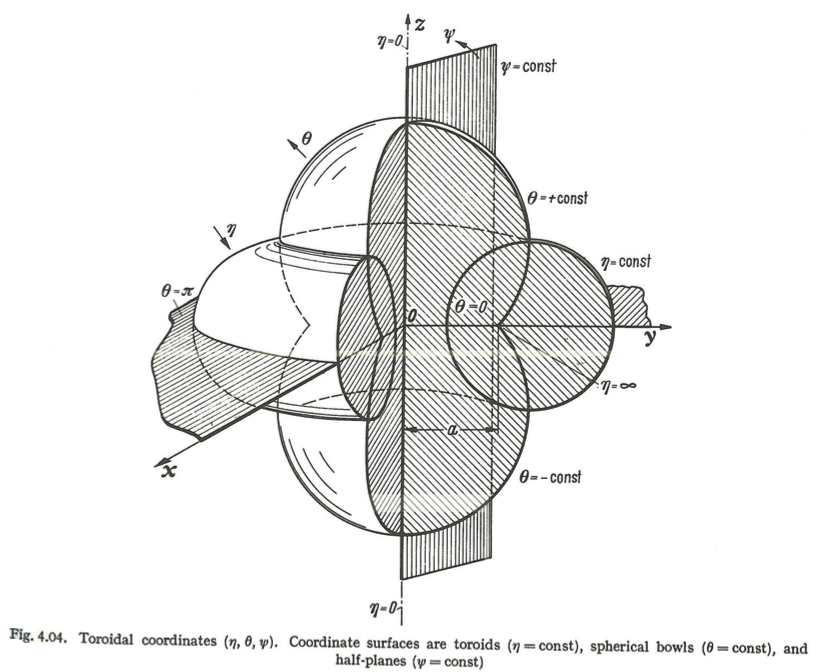
\includegraphics[scale=0.55,natwidth=824,natheight=672, angle=1
]{../figures/toroidal_coordinates.png} 
\caption[Coordinate surfaces for toriodal coordinates.]{Coordinate surfaces for toriodal 
coordinates. Picture scanned from \cite{MS71}.}
\label{fig:toroidal_surfaces}
\end{figure}

\hspace{-6mm}In the $xy$-plane the focal ring(also known as the 
\emph{reference circle}) has radius a. The $\eta$ coordinate is given as the following ratio
\begin{align*}
\eta = \ln \frac{d_1}{d_2}.
\end{align*} 
The coordinates vary as following :
\begin{align*}
\left\{\begin{matrix}
 -\pi& <& \theta &<& \pi,\\
 0 &\leq& \psi &<& 2\pi,\\
& \phantom{0} & \eta &\geq& 0.
\end{matrix}\right.
\end{align*}

Our first task is to determine the metric (found from the transformation between cartesian 
and toroidal coordinates), which is given as 
\begin{align*}
g_{ij} = \frac{\partial \mathbf{r}}{\partial u_i} \cdot \frac{\partial \mathbf{r}}{\partial u_j},
\end{align*}
where $u_i = (\eta, \theta , \psi)$, for $i=1,2,3$, and $\mathbf{r}$ is the vector
\begin{align*}
\mathbf{r} = x\hat{\mathbf{e}}_1 + y\hat{\mathbf{e}}_2 + z\hat{\mathbf{e}}_3 = 
x(\eta, \theta , \psi)\hat{\mathbf{e}}_1 + y(\eta, \theta , \psi)\hat{\mathbf{e}}_2 + 
z(\eta, \theta , \psi)\hat{\mathbf{e}}_3
\end{align*}
spanned by cartesian orthogonal basis\footnote{Which has the property 
$\hat{e}_i\cdot \hat{e}_j = \delta_{ij}$, and any derivation of the basis is identically zero.
Which becomes quite practical when attempting to find the metric.}. 
We can find all the components of the metric by hand calculations, or through Python using 
the symbolic package SymPy (see Appendix \ref{appendix:find_metric}). 

The entries of the metric $g_{ij}$ are found from change of coordinates when applying the 
equations \eqref{eq:x_coord}-\eqref{eq:z_coord}. The only non-zero entries are found to be 
the diagonal entries, i.e $i=j$. Which are given as
\begin{align*}
g_{11} &= \frac{\partial \mathbf{r}}{\partial u_1} \cdot \frac{\partial \mathbf{r}}{\partial u_1} 
	    = \frac{\partial \mathbf{r}}{\partial \eta} \cdot \frac{\partial \mathbf{r}}{\partial \eta} \\
 	 & =  \frac{\partial (x\hat{\mathbf{e}}_1 + y\hat{\mathbf{e}}_2 + 
		z\hat{\mathbf{e}}_3)}{\partial \eta} \cdot \frac{\partial (x\hat{\mathbf{e}}_1 +
	         y\hat{\mathbf{e}}_2 + z\hat{\mathbf{e}}_3)}{\partial \eta} \\
	 & = \left[\frac{\partial x}{\partial \eta} \right]^2 + \left[\frac{\partial y}{\partial \eta} \right]^2
		+ \left[\frac{\partial z}{\partial \eta} \right]^2.
\end{align*}
Similarly, the other non-zero entries of the metric are 
\begin{align*}
g_{22} &= \left[\frac{\partial x}{\partial \theta} \right]^2 + \left[\frac{\partial y}{\partial \theta} \right]^2
	    + \left[\frac{\partial z}{\partial \theta} \right]^2, \qquad\qquad\\
g_{33} &= \left[\frac{\partial x}{\partial \psi} \right]^2 + \left[\frac{\partial y}{\partial \psi} \right]^2
	    + \left[\frac{\partial z}{\partial \psi} \right]^2.
\end{align*}
Here we list the calculations necessary to find $g_{11}$. The other entries of $g_{ij}$ are found by
using the same techniques as demonstrated here.
\begin{align*}
\frac{\partial x}{\partial \eta} &= \frac{a \cos(\psi) [1 - \cosh(\eta)\cos(\theta)]}
						    {[\cosh(\eta) - \cos(\theta)]^2} \\
&\Downarrow \\
\left[\frac{\partial x}{\partial \eta} \right]^2 &= \frac{a^2 \cos^2(\psi) [1 - \cosh(\eta)\cos(\theta)]^2}
								    {[\cosh(\eta) - \cos(\theta)]^4}
\end{align*}
Similary, we find the other expressions
\begin{align*}
\left[\frac{\partial y}{\partial \eta} \right]^2 &= \frac{a^2 \sin^2(\psi) [1 - \cosh(\eta)\cos(\theta)]^2}
								    {[\cosh(\eta) - \cos(\theta)]^4}, \\
\left[\frac{\partial z}{\partial \eta} \right]^2 &= \frac{a^2\sinh^2(\eta)\sin^2(\theta)}
								    {[\cosh(\eta) - \cos(\theta)]^4}.
\end{align*}
Adding all the terms together,
\begin{align*}
g_{11} &= \frac{a^2 \cos^2(\psi) [1 - \cosh(\eta)\cos(\theta)]^2 + 
		       a^2 \sin^2(\psi) [1 - \cosh(\eta)\cos(\theta)]^2 +
		       a^2\sinh^2(\eta)\sin^2(\theta)}
	     	    {[\cosh(\eta) - \cos(\theta)]^4} \\ 
	  &= a^2\left(\frac{1  -  2\cosh(\eta)\cos(\theta) + \cosh^2(\eta)\cos^2(\theta)+ 
			    [1 - \cos^2(\theta)]\sinh^2(\eta)}
		            {[\cosh(\eta) - \cos(\theta)]^4}\right)\\
	  &= a^2\left(\frac{\cosh^2(\eta) - 2\cosh(\eta)\cos(\theta) + \cos^2(\theta)}
		            {[\cosh(\eta) - \cos(\theta)]^4}\right)
\end{align*}
where we have used the trignometric identities $\sin^2 (\psi) + \cos^2 (\psi) = 
\sin^2 (\theta) + \cos^2 (\theta) = 1$, and $\cosh^2(\eta) - \sinh^2(\eta) = 1$. We can simplify
this expression further, by expanding the factor $[\cosh(\eta) - \cos(\theta)]^2 = \cosh^2(\eta)
- 2\cosh(\eta)\cos(\theta) + \cos^2(\theta)$. Hence, we end up with the first entry of the metric,
\begin{align}
\label{eq:g11}
g_{11} = \frac{a^2}{[\cosh(\eta) - \cos(\theta)]^2}.
\end{align}
The other diagonal entries (i.e the non-zero entries of $g_{ij}$) are found to be
\begin{align}
\label{eq:g22}
g_{22} = g_{11} &= \frac{a^2}{[\cosh(\eta) - \cos(\theta)]^2},
\\
\label{eq:g33}
g_{33} &= \frac{a^2\sinh^2(\eta)}{[\cosh(\eta) - \cos(\theta)]^2}.
\end{align}
\\

Now we can find the Christoffel symbols for our metric $g_{ij}$, and thereby be able to 
determine the Riemann curvature tensor. The process is as following :
\begin{enumerate}
\item Determine the non-zero contributions from Equation \eqref{eq:first_kind}
\item Determine the non-zero contributions from Equation 
\eqref{eq:second_kind}\footnote{Notice that the conjugate metric $g^{ij}$ is relatively 
easy to determine when the metric is diagonal. The entries of the conjugate metric 
become the inverse of the entries of $g_{ij}$.}
\item Finally determine all the derivatives in Equation \eqref{eq:RCT}
\end{enumerate}

\hspace{-6mm}Here are points (1) and (2) :
In order determine all the terms of the Riemann curvature tensor we must determine the Christoffel
symbols of second kind, which again implies that we must determine the corresponding Christoffel
symbols of first kind. For the sake of clarity, we restate the Riemann curvature tensor
\begin{align}
\label{eq:RCT_}
R^m_{\phantom{m}ijk} =  
\frac{\partial}{\partial x^j}{m \brace i\,\,k} - \frac{\partial}{\partial  x^k}{m \brace i\,\,j} 
+ {n \brace i\,\,k}{m \brace n\,\,j} - {n \brace i\,\,j}{m \brace n\,\,k},
\end{align}
Let us initially focus on the first term here
\begin{align}
 \frac{\partial}{\partial x^j}{m \brace i\,\,k}.
\end{align}
Using the definition for Christoffel symbol of second kind \eqref{eq:second_kind}, and inserting for 
the first kind \eqref{eq:first_kind}, we get the following expression
\begin{align}
 \frac{\partial}{\partial x^j}{m \brace i\,\,k} &=  \frac{\partial}{\partial x^j}\, g^{mk} 
 \left[a i,k\right]\\
\label{eq:first_term_RCT}
&= \frac{1}{2}\frac{\partial}{\partial x^j} \, g^{mk} \left(\frac{\partial g_{ak}}{\partial x^i} + 
\frac{\partial g_{ki}}{\partial x^a} - \frac{\partial g_{ai}}{\partial x^k}\right)
\end{align}
for $a,i,k,m = 1,2,3$, and where the coordinates are $x^i = \eta , \theta, \psi$, for $i = 1,2,3$.

There are three cases where we get contribution from the Equation \eqref{eq:first_term_RCT}.
\begin{itemize}
\item Case 1, where $m=k$, and $a=k$,
\item Case 2, where $m=k$, and $i=k$,
\item Case 3, where $m=k$, and $i=a$.
\end{itemize}
For every case we require that $m=k$. This is because the conjugate metric $g^{mk}$ is zero every
where except on the diagonal. As $g^{mk} = (g_{mk})^{-1}$, we find conjugate metric by 
inverting the entries of $g_{mk}$.

For Case 1, we get the following expression
\begin{align*}
\frac{1}{2}\frac{\partial}{\partial x^j} \, g^{mk} \left(\frac{\partial g_{ak}}{\partial x^i} + 
\frac{\partial g_{ki}}{\partial x^a} - \frac{\partial g_{ai}}{\partial x^k}\right) &=
\frac{1}{2}\frac{\partial}{\partial x^j} \, g^{kk} \left(\frac{\partial g_{kk}}{\partial x^i} + 
\frac{\partial g_{ki}}{\partial x^k} - \frac{\partial g_{ki}}{\partial x^k}\right)  
\nonumber
\\
&= \frac{1}{2}\frac{\partial}{\partial x^j} \left( g^{kk} \frac{\partial g_{kk}}{\partial x^i}\right)
\end{align*}
Similarly, for the other two cases we get the expressions
\begin{align*}
\mbox{Case 2 : } &\, m=k, \qquad i=k \nonumber
\\
\frac{1}{2}\frac{\partial}{\partial x^j} \, g^{mk} \left(\frac{\partial g_{ak}}{\partial x^i} + 
\frac{\partial g_{ki}}{\partial x^a} - \frac{\partial g_{ai}}{\partial x^k}\right) &=
\frac{1}{2}\frac{\partial}{\partial x^j} \, g^{kk} \left(\frac{\partial g_{ak}}{\partial x^k} + 
\frac{\partial g_{kk}}{\partial x^a} - \frac{\partial g_{ak}}{\partial x^k}\right) 
\nonumber
\\
&= \frac{1}{2}\frac{\partial}{\partial x^j} \left( g^{kk} \frac{\partial g_{kk}}{\partial x^a}\right)
\\
\mbox{Case 3 : } &\, m=k, \qquad i=a \nonumber
\\
\frac{1}{2}\frac{\partial}{\partial x^j} \, g^{mk} \left(\frac{\partial g_{ak}}{\partial x^i} + 
\frac{\partial g_{ki}}{\partial x^a} - \frac{\partial g_{ai}}{\partial x^k}\right) &=
\frac{1}{2}\frac{\partial}{\partial x^j} \, g^{kk} \left(\frac{\partial g_{ik}}{\partial x^i} + 
\frac{\partial g_{ki}}{\partial x^i} - \frac{\partial g_{ii}}{\partial x^k}\right) 
\nonumber
\\
&= \frac{1}{2}\frac{\partial}{\partial x^j} \left( g^{kk} \frac{\partial g_{kk}}{\partial x^i}\right)
\end{align*}
Adding the results from all three of the cases, we get the result
\begin{align}
\frac{\partial}{\partial x^j}{m \brace i\,\,k} =
\frac{\partial}{\partial x^j} \left(g^{kk} \frac{\partial g_{kk}}{\partial x^i} + \frac{1}{2}g^{kk}\frac{\partial g_{kk}}{\partial x^a}\right)
\end{align}
The other terms of the Riemann tensor \eqref{eq:RCT_} give corresponding terms
\begin{align}
-\frac{\partial}{\partial  x^k}{m \brace i\,\,j} &= 
-\frac{\partial}{\partial x^k} \left(g^{jj} \frac{\partial g_{jj}}{\partial x^i} - \frac{1}{2}g^{jj}\frac{\partial g_{jj}}{\partial x^a}\right) \\
{n \brace i\,\,k}{m \brace n\,\,j} &= 
\left(g^{kk} \frac{\partial g_{kk}}{\partial x^i} + \frac{1}{2}g^{kk}\frac{\partial g_{kk}}{\partial x^a}\right)
\left(g^{jj} \frac{\partial g_{jj}}{\partial x^a} + \frac{1}{2}g^{jj}\frac{\partial g_{jj}}{\partial x^i}\right)\\
- {n \brace i\,\,j}{m \brace n\,\,k} &=
- \left(g^{jj} \frac{\partial g_{jj}}{\partial x^i} + \frac{1}{2}g^{jj}\frac{\partial g_{jj}}{\partial x^a}\right)
\left(g^{kk} \frac{\partial g_{kk}}{\partial x^a} + \frac{1}{2}g^{kk}\frac{\partial g_{kk}}{\partial x^j}\right)
\end{align}
We see that, for $i = j = k = a = 3$, every term becomes zero (as the respective derivatives are zero). For every other
permutation, each term cancels the other, resulting in that every element of the Riemann curvature tensor is zero for
the toroidal coordinates. Implying that this is a flat space. 
\end{document}